\begin{thm}{003}{\hosi 8}{}
 半円$\mr{C}$: $x^2+y^2=1,\, y>0$に第一象限の点Pで接する直線$\ell$がある。点$\mr{A}(-1,0)$を通り、$\ell$に直交する直線と$\mr{C}$の交点を$\mr{B}$とし、弦$\mr{AB}$, $\mr{AP}$と弧$\mr{BP}$で囲まれた図形を$\mr{D}$とする。$\mr{D}$を$\ell$の周りに一回転させてできる図形の体積$V$を最大にするような$\mr{P}$の座標を求めよ。
\end{thm}

\begin{figure}[H]
 \centering
 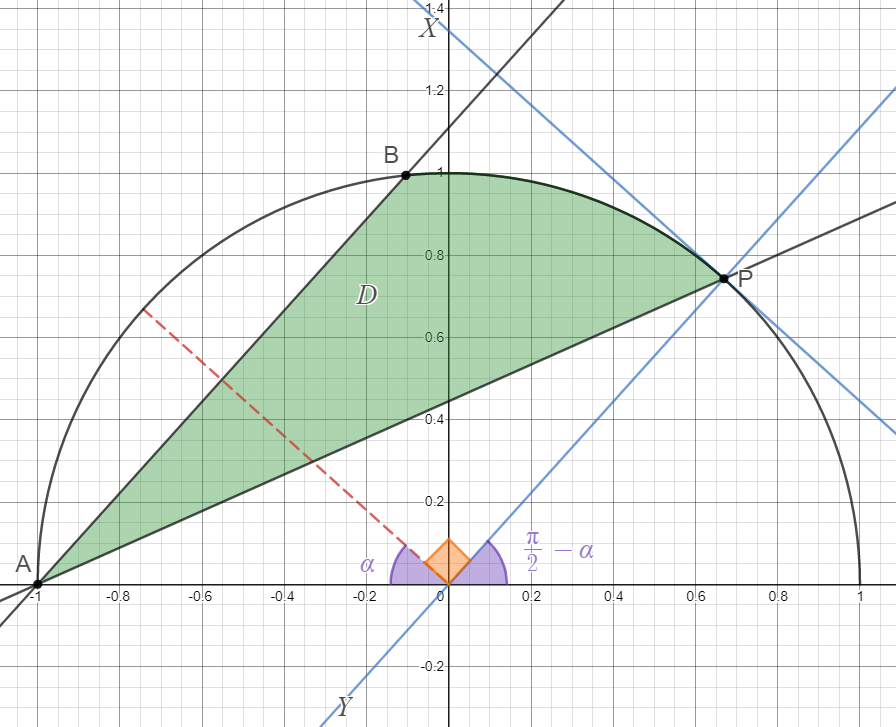
\includegraphics[width=0.7\linewidth]{../problems/Q_003/A_003_1.png}
\end{figure}

図のように角度$\alpha$を定める。点$\mr{P}$が第一象限を動くとき、$\alpha$は$0<\alpha<\dfrac{\pi}{2}$の範囲を動く。また、点$\mr{P}$を原点とする$X, Y$座標を青線のように設定する。この座標の下では、図は次のようになる。

\begin{figure}[H]
 \centering
 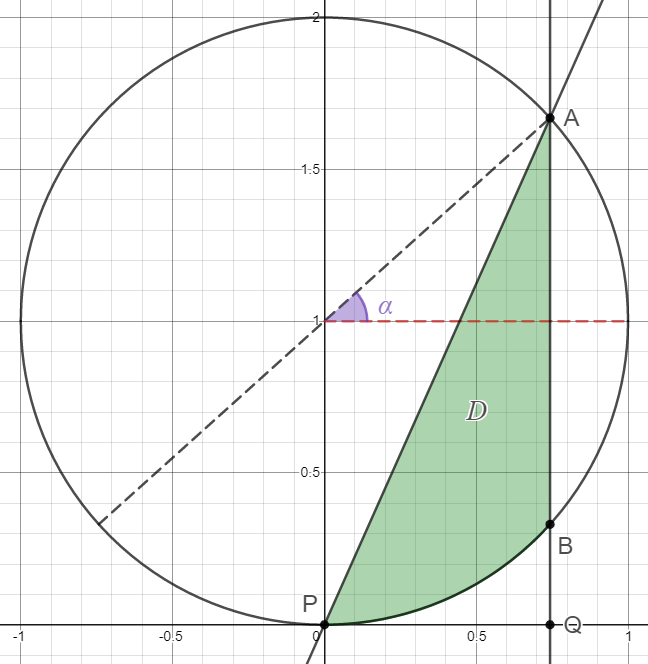
\includegraphics[width=0.6\linewidth]{../problems/Q_003/A_003_2.png}
\end{figure}

以下この座標系において考える。このもとで$\mr{A}(\cos\alpha, 1+\sin\alpha)$, $\mr{B}(\cos\alpha, 1-\sin\alpha)$となる。また弧$\mr{BP}$は$Y=1-\sqrt{1-X^2}$ (ただし$0\le X\le \cos\alpha$) となる。点$\mr{Q}(\cos\alpha, 0)$をおく。回転体の体積$V$は、$\triangle\mr{APQ}$の回転体(円錐)から線分$\mr{PQ, BQ}$と弧$\mr{BP}$で囲まれた領域の回転体を除くことで得られるから、
\begin{align*}
 V&=\frac{\pi}{3}(1+\sin\alpha)^2\cos\alpha-\pi\int_0^{\cos\alpha}\!(1-\sqrt{1-X^2})^2 \,dX
\end{align*}
これを$\alpha$で微分して、
\begin{align*}
 \left(\frac{3}{\pi}V\right)'&=2(1+\sin\alpha)\cos^2\alpha+(1+\sin\alpha)^2(-\sin\alpha) \\
 &\qquad -3(1-\sqrt{1-\cos^2\alpha})^2(-\sin\alpha) \\
 &=-2(5\sin^2\alpha-2\sin\alpha-1)
\end{align*}
となる。よって$V'=0$となるのは$\sin\alpha=\dfrac{1\pm\sqrt{6}}{5}$のときであるが、$0<\alpha<\dfrac{\pi}{2}$では$\sin\alpha>0$であるから複合は正のみ適する。加えてこの範囲において$\sin\alpha$は単調増加であるから、$\alpha$の増加とともに$V'$の符号は負から正へ転じるので、$\sin\alpha=\dfrac{1+\sqrt{6}}{5}$となるときに$V$は極大となる。

このとき、点$\mr{P}$の座標は$xy$座標で$\mr{P}\left(\cos\left(\frac{\pi}{2}-\alpha\right), \sin\left(\frac{\pi}{2}-\alpha\right)\right)$となる。
\begin{align*}
 \cos\left(\frac{\pi}{2}-\alpha\right)&=\sin\alpha=\frac{1+\sqrt{6}}{5} \\
 \sin\left(\frac{\pi}{2}-\alpha\right)&=\cos\alpha=\frac{\sqrt{18-2\sqrt{6}}}{5}
\end{align*}
であるから、求める点$\mr{P}$の座標は
\[ \mr{P}\left(\frac{1+\sqrt{6}}{5}, \frac{\sqrt{18-2\sqrt{6}}}{5}\right) \]
